\documentclass[12pt]{article}

% Packages
\usepackage[margin=1.2in]{geometry}
\usepackage{graphicx}
\usepackage{placeins}
\usepackage{enumerate}
\usepackage{colortbl}
\usepackage{listings}
\usepackage{titling}
\usepackage{tabularx}
\usepackage{longtable}
\usepackage{booktabs}
\usepackage{hyperref}
\usepackage{makecell}
\usepackage{caption}
\usepackage{array}
\usepackage[parfill]{parskip}

% Comments --------------------------------------------------------------------
\usepackage{xcolor}
\newif\ifcomments\commentstrue
\ifcomments \newcommand{\authornote}[3]{\textcolor{#1}{[#3 ---#2]}}
\newcommand{\todo}[1]{\textcolor{red}{[TODO: #1]}} \else
\newcommand{\authornote}[3]{} \newcommand{\todo}[1]{} \fi
\newcommand{\wss}[1]{\authornote{magenta}{SS}{#1}}
\newcommand{\ds}[1]{\authornote{blue}{DS}{#1}}
% End Comments ---------------------------------------------------------------

% Formatting
\setlength{\parindent}{0pt}
\captionsetup[table]{skip=2pt}

% Title Page -----------------------------------------------------------------
\title{
\LARGE GEANT-4 GPU Port:
\\\vspace{10mm}
\large \textbf{Design Document: System Architecture}
\vspace{40mm}
}
\author{
\textbf{Team 8}
\\Stuart Douglas -- dougls2
\\Matthew Pagnan -- pagnanmm
\\Rob Gorrie -- gorrierw
\\Victor Reginato -- reginavp
\vspace{10mm}
}
\date{\vfill \textbf{System Architecture: Version 0}\\ \today}
% End Title Page -------------------------------------------------------------

% ============================== BEGIN DOCUMENT ============================= %
\begin{document}
\pagenumbering{gobble} % start numbering after TOC

% ============================== Title Page ============================= %
\maketitle
\newpage

% ================================= TOC ================================= %
\renewcommand{\contentsname}{Table of Contents}
\tableofcontents
\newpage
\pagenumbering{arabic}

\section{Introduction}% ============== Matt
\subsection{Revision History}
All major edits to this document will be recorded in the table below.

\begin{table}[h]
\centering
\caption{Revision History}\label{Table_Revision}
\begin{tabularx}{\textwidth}{Xll}
\toprule
\bf Description of Changes & \bf Author & \bf Date\\\midrule
\arrayrulecolor{lightgray}
Set up sections and filled out Introduction section & Matthew & 2015-12-15\\\hline
Document structure adjustments & Stuart & 2016-1-8\\\hline
Filled out Likely/Unlikely Changes section & Rob & 2016-1-9\\
\arrayrulecolor{black}
\bottomrule
\end{tabularx}
\end{table}

\subsection{Terms Used}
\begin{table}[h]
\centering
\caption{Glossary}\label{Table_Glossary}
\begin{tabularx}{\textwidth}{lX}
\toprule
\bf Term & \bf Description\\\midrule
\arrayrulecolor{lightgray}
Geant4 & open-source software toolkit for simulating particle interactions\\\hline
G4-STORK & fork of Geant4 developed by McMaster's Engineering Physics department to simulate McMaster's nuclear reactor\\\hline
GPU & graphics processing unit, well-suited to parallel computing tasks\\\hline
CPU & computer processing unit, well-suited to serial tasks\\\hline
CUDA & parallel computing architecture for GPU programming, developed by NVIDIA\\\hline
CUDA file & text file with .cu extension that includes host code (which runs on the CPU) and device code (which runs on the GPU)\\\hline
NVIDIA & computer hardware and software company specializing in GPU's\\\hline
Host & the CPU and its memory, managed from within a CUDA file, sends and receives data to the GPU\\\hline
Device & the GPU and its memory, managed from the host, performs computations requested by the host\\
\arrayrulecolor{black}
\bottomrule
\end{tabularx}
\end{table}

\subsection{List of Tables}
\begin{center}
\begin{tabular}{cl}
\toprule
\bf Table \# & \bf Title\\\midrule
\arrayrulecolor{lightgray}
\ref{Table_Revision} & Revision History\\\hline
\ref{Table_Glossary} & Glossary\\\hline
\ref{Table_Figures}  & List of Figures\\\hline
\ref{Table_GPUIntegration} & Comparison of GPU Integration Approaches\\\hline
\ref{Table_LikelyChangesAndDesign} & Relationship Between Likely Changes and Design\\\hline
\ref{Table_RequirementsAndDesign} & Traceability of Requirements and Design\\
\arrayrulecolor{black}
\bottomrule
\end{tabular}
\end{center}

\subsection{List of Figures}

\begin{table}[h]
\centering
\caption{List of Figures}\label{Table_Figures}
\begin{tabular}{cl}
\toprule
\bf Figure \# & \bf Title\\\midrule
\ref{imgUsesHierarchy} & Uses Hierarchy for G4NeutronHPVector\\
\bottomrule
\end{tabular}
\end{table}

\section{Overview}
\subsection{Purpose of Project}
The purpose of the project is to reduce the computation times of particle simulations in Geant4 by parallelizing and running certain procedures on the GPU. The main stakeholders are members of McMaster's department of Engineering Physics that use Geant4 to simulate particle interactions in McMaster's nuclear reactor.

\subsection{Description}
The project aims to improve the computation times of Geant4 particle simulations by running certain parallel operations on a GPU. GEANT4-GPU will be a fork of the existing Geant4 system with the additional option for users with compatible hardware to run operations on the GPU for improved performane. This functionality will be available on Mac, Linux and Windows operating systems running on computers with NVIDIA graphics cards that support CUDA.

The design strategy for the project will be based on taking a specific, computationally heavy class from Geant4 and creating a class that fulfills the same interface but that runs on the GPU. This will be repeated for many classes until the project's deadline has been reached. The user will have the option of using the existing classes (running on the CPU) or the new ones (running on the GPU).

\subsection{Document Structure \& Template}
The design documentation for the project is based off of WHAT TEMPLATES?????? and is broken into two main documents.

This system architecture document details the system architecture, including an overview of the modules that make up the system, analysis of aspects that are likely and unlikely to change, reasoning behind the high-level decisions, and a table showing how each requirement is addressed in the proposed design.

A separate detailed design document covers the specifics of several key modules in the project. This includes the interface specification and implementation decisions.

\section{Important Design Decisions \& Reasoning}
\subsection{GPU Computing for Geant4}\label{Sec_WhyGPU}
Geant4 simulations typically involve simulating the movement of many particles (up to millions). Each particle has its new state (postition, energy etc.) calculated at each timestep independently of the other particles. Each state update requires serially traversing an array of particles and performing calculations on each.

This problem is well-suited to parallelization, as each particle has the same, relatively simple functions applied to it independently. Although not faster in many cases, when massive parallelization is possible, running on the GPU can lead to significant performance improvements. This led the stakeholders to propose using the GPU to do some calculations in Geant4 with the goal of reducing the runtime of the simulations.

\subsection{CUDA}
The two most popular software libraries for performing general computing tasks on the CPU are CUDA and OpenCL. The decision was made to use CUDA for a variety of reasons. Developed by NVIDIA, CUDA has more extensive documentation than OpenCL, a larger online community, a more consistent interface, integration with CMake (the Geant4 build system), and several researchers have successfully integrated small parts of Geant4 with CUDA.

There are two main disadvantages of CUDA however that are worth discussing. First and foremost, CUDA programs can only run on NVIDIA GPUs. If the user has a GPU made by a different manufacturer, they will not be able to receive any of the performance benefits of the new product. This was determined to be acceptable as the stakeholders explicitly stated plans to purchase a NVIDIA GPU, and McMaster's GPU servers all use NVIDIA graphics cards. Secondly, while OpenCL is open-source, CUDA is proprietary and owned by NVIDIA (although distributed as freeware). This is not optimal, however it was decided that the advantages of the larger community and consistent interface outweighed the disadvantages of a non-open-source library.

\subsection{GPU Integration Approach}\label{Sec_IntegrationApproach}
When considering how to integrate the GPU computations with the non-ported procedures that run on the CPU there were five main options (option 5 was chosen):
\begin{enumerate}
\item Port entire Geant4 toolkit to fully run on the GPU.
\item Port all functions of some classes to run on the GPU, those classes will only be instantiated in GPU memory.
\item Port some functions of some classes to run on the GPU, those classes will be stored only in main memory. Data required by the GPU functions will be passed from the host.
\item Port some functions of some classes to run on the GPU, those classes will be stored in main memory and a copy will be stored in GPU memory. Updates to the state will be applied to both copies.
\item Port some functions of some classes to run on the GPU, those classes will have some data stored in main memory and some (different) data stored in GPU memory. If data is required by a function running on the CPU that is stored on the GPU (or vice versa), a copy of the data will be received through a getter function.
\end{enumerate}

\begin{table}
\centering
\caption{Comparison of GPU Integration Approaches}\label{Table_GPUIntegration}
\begin{tabularx}{\textwidth}{cXX}
\toprule
\bf Option & \bf Pros & \bf Cons\\\midrule
\arrayrulecolor{lightgray}

1 & \textbullet $\,$ largest speedup as all aspects of system would be parallelized
  & \textbullet $\,$ far beyond scope of project and resources available\\\hline

2 & \textbullet $\,$ no memory usage penalty as class only instantiated once\newline
    \textbullet $\,$ no performance penalty for passing data from main memory to GPU memory
  & \textbullet $\,$ difficult to use existing code if GPU computation disabled\newline
    \textbullet $\,$ requires porting all functions of class to GPU even if functions won't give large performance benefits\newline
    \textbullet $\,$ smaller memory available for GPU may mean that less particles can be simulated at once\\\hline

3 & \textbullet $\,$ no memory usage penalty as class only instantiated once\newline
    \textbullet $\,$ easily interfaces with existing codebase\newline
    \textbullet $\,$ easy to use existing code if GPU computation disabled\newline
    \textbullet $\,$ doesn't require porting functions to GPU that will not have large performance benefits
  & \textbullet $\,$ all data must be passed from main memory to GPU memory every function call\\\hline

4 & \textbullet $\,$ no performance penalty for passing data between main memory and GPU memory\newline
    \textbullet $\,$ easily interfaces with existing codebase\newline
    \textbullet $\,$ easy to use existing code if GPU computation disabled\newline
    \textbullet $\,$ doesn't require porting functions to GPU that will not have large performance benefits
  & \textbullet $\,$ double the memory usage\newline
    \textbullet $\,$ smaller memory available for GPU may mean that less particles can be simulated at once\newline
    \textbullet $\,$ everytime state updated it must be updated twice\\\hline

5 & \textbullet $\,$ reduced performance penalty for passing data between main memory and GPU memory\newline
    \textbullet $\,$ easy to use existing code if GPU computation disabled\newline
    \textbullet $\,$ easily interfaces with existing codebase\newline
    \textbullet $\,$ doesn't require porting functions to GPU that will not have large performance benefits
  & \textbullet $\,$ performance penalty if data required by CPU from GPU memory (or vice versa)\\

\arrayrulecolor{black}
\bottomrule
\end{tabularx}
\end{table}
\clearpage

In all options except 1 and 2, a function call to one of the functions of a ported class will be received by the existing C++ class, which will then either execute the existing code if that function has not been ported or if GPU computation is disabled, or will call the corresponding function from the CUDA file.

Option 5 was chosen due to its ability to divide work easily, its compatibility with the current codebase, and the memory advantages over option 4.

\subsection{G4NeutronHPVector}\label{subsec_G4NeutronHPVector} % rob
As was explained in the preceding subsection, the problem has been decomposed to that of only integrating specific functions from given modules with the CUDA technology. With that said, a decision needed to be made as for which class and which functions within that class to integrate.

G4HPNeutronVector was chosen to port to the GPU for two main reasons. The first is that this decision was made to satisfy system and technical requirements, and the second is a matter of satisfying client requirements.

Geant4 organizes the processes for particles that it must manipulate into separate classes. These classes house functions appropriate to the mechanics surrounding those particles. These classes are the target for parallelization because they are where large arrays of particles and data are stored and manipulated (note: these are not the classes that represent the particles themselves, but the classes that store the functions germane to the given class of particles). These classes are referred to as models in the Geant4 code base. There are over 100 of these `models' under the hadronic category alone (hadronic particles are those composed of quarks). The problem now is reduced to deciding which model(s) to integrate with the CUDA technology.
	 
The decision as to which model to integrate was made to satisfy client requirements. The problem at hand was proposed by Dr. Buijs and his graduate students from the Engineering Physics department at McMaster. Dr. Buijs' team uses Geant4 to model the university's local nuclear reactor. Their simulations very heavily depend on manipulating neutrons through the G4NeutronHPVector class. Therefore, this model was chosen for CUDA integration in an attempt to offer the most significant performance increases to Dr. Buijs and his students specifically.

\section{Likely and Unlikely Changes}
Different aspects of the system are presented below in two lists, those that are likely to change in the future and those that are unlikely to change. Relative likelihood of changes in the same category may vary.

Following the lists of likely and unlikely changes, the relationship between likely changes and design components is presented.

\subsection{Likely Changes}\label{Sec_LikelyChanges} %========== Rob
\begin{enumerate}
\item Parallelizing other modules in addition to G4NeutronHPVector
\item The serial, CPU-bound algorithms used by Geant4 will likely not be suited to running on the GPU
\item Specifics of CMake implementation to compile and link CUDA code
\end{enumerate}

\subsection{Unlikely Changes} %========= Rob
\begin{enumerate}
\item Using CUDA as GPU programming library
\item Using the GPU to run certain computations in parallel
\item The command-line interface of Geant4
\item The use of CMake as the build system
\item Additions of any new process or model modules to Geant4
\item Enabling/disabling CUDA using CMake flag
\end{enumerate}

\subsection{Traceability of Likely Changes to Design Components}
The following table addresses all likely changes discussed above and their relationship to the design of the system. All numbers in the ``Change'' column refer to the enumeration from the ``Likely Changes'' list (section \ref{Sec_LikelyChanges})

\begin{center}
\begin{longtable}{c >{\raggedright\arraybackslash}p{0.7\textwidth}}

\caption{Likely Changes and Design Relationship}\label{Table_LikelyChangesAndDesign}
\\\toprule
\bf Change & \bf Design Component\\\toprule
\arrayrulecolor{lightgray}

1 & Deciding which process model to parallelize (see \ref{subsec_G4NeutronHPVector}, paragraph 3)\\\hline
2 & CMake module\\\hline
3 & Deciding which functions in model classes to parallelize\\\hline
\arrayrulecolor{black}
\bottomrule
\end{longtable}
\end{center}

\section{Module Hierarchy}%============= Stuart
\subsection{Decomposition of Components}
The project is based off of Geant4, an existing software system, and modifying specific modules of that system. As such, the decomposition used by the existing system will match the modules of the new system in the project development.

Each module in Geant4 is represented by a C++ class, and the project will port a subset of said classes to the GPU. The decision of which classes to port is derived from performance analysis of the program, with the most computationally time-consuming classes being the targets, such as G4NeutronHPVector (see section \ref{subsec_G4NeutronHPVector}). Furthermore, it is possible that not all functions of the class will be ported. The focus will be on porting ``clean'' (having a limited number of side effects), computationally heavy functions. This allows the work to be broken down on a class-by-class and function-by-function basis, and completing the port of one class does not depend on any other classes being ported. If a function running on the GPU requires an external module, the C++ host code for the CUDA that interfaces with the GPU will extract and pass any required information to the GPU and perform any state updates.

\subsection{Uses Hierarchy}
Since each modified module of the project will have a direct 1-to-1 relationship with an existing module in Geant4, the uses hierarchy with the new, GPU-enabled classes will be identical to the existing uses hierarchy of Geant4 with their corresponding existing classes.

Geant4 is an extremely large system with many modules, so its entire uses hierarchy will not be documented here. Instead, the following hierarchy shows the dependencies of the G4NeutronHPVector module, which is currently the focus of the project. Note that modules used by system libraries are not included, but the system libraries themselves are included.

\begin{figure}[h]
\caption{Uses Hierarchy for G4NeutronHPVector}\label{imgUsesHierarchy}
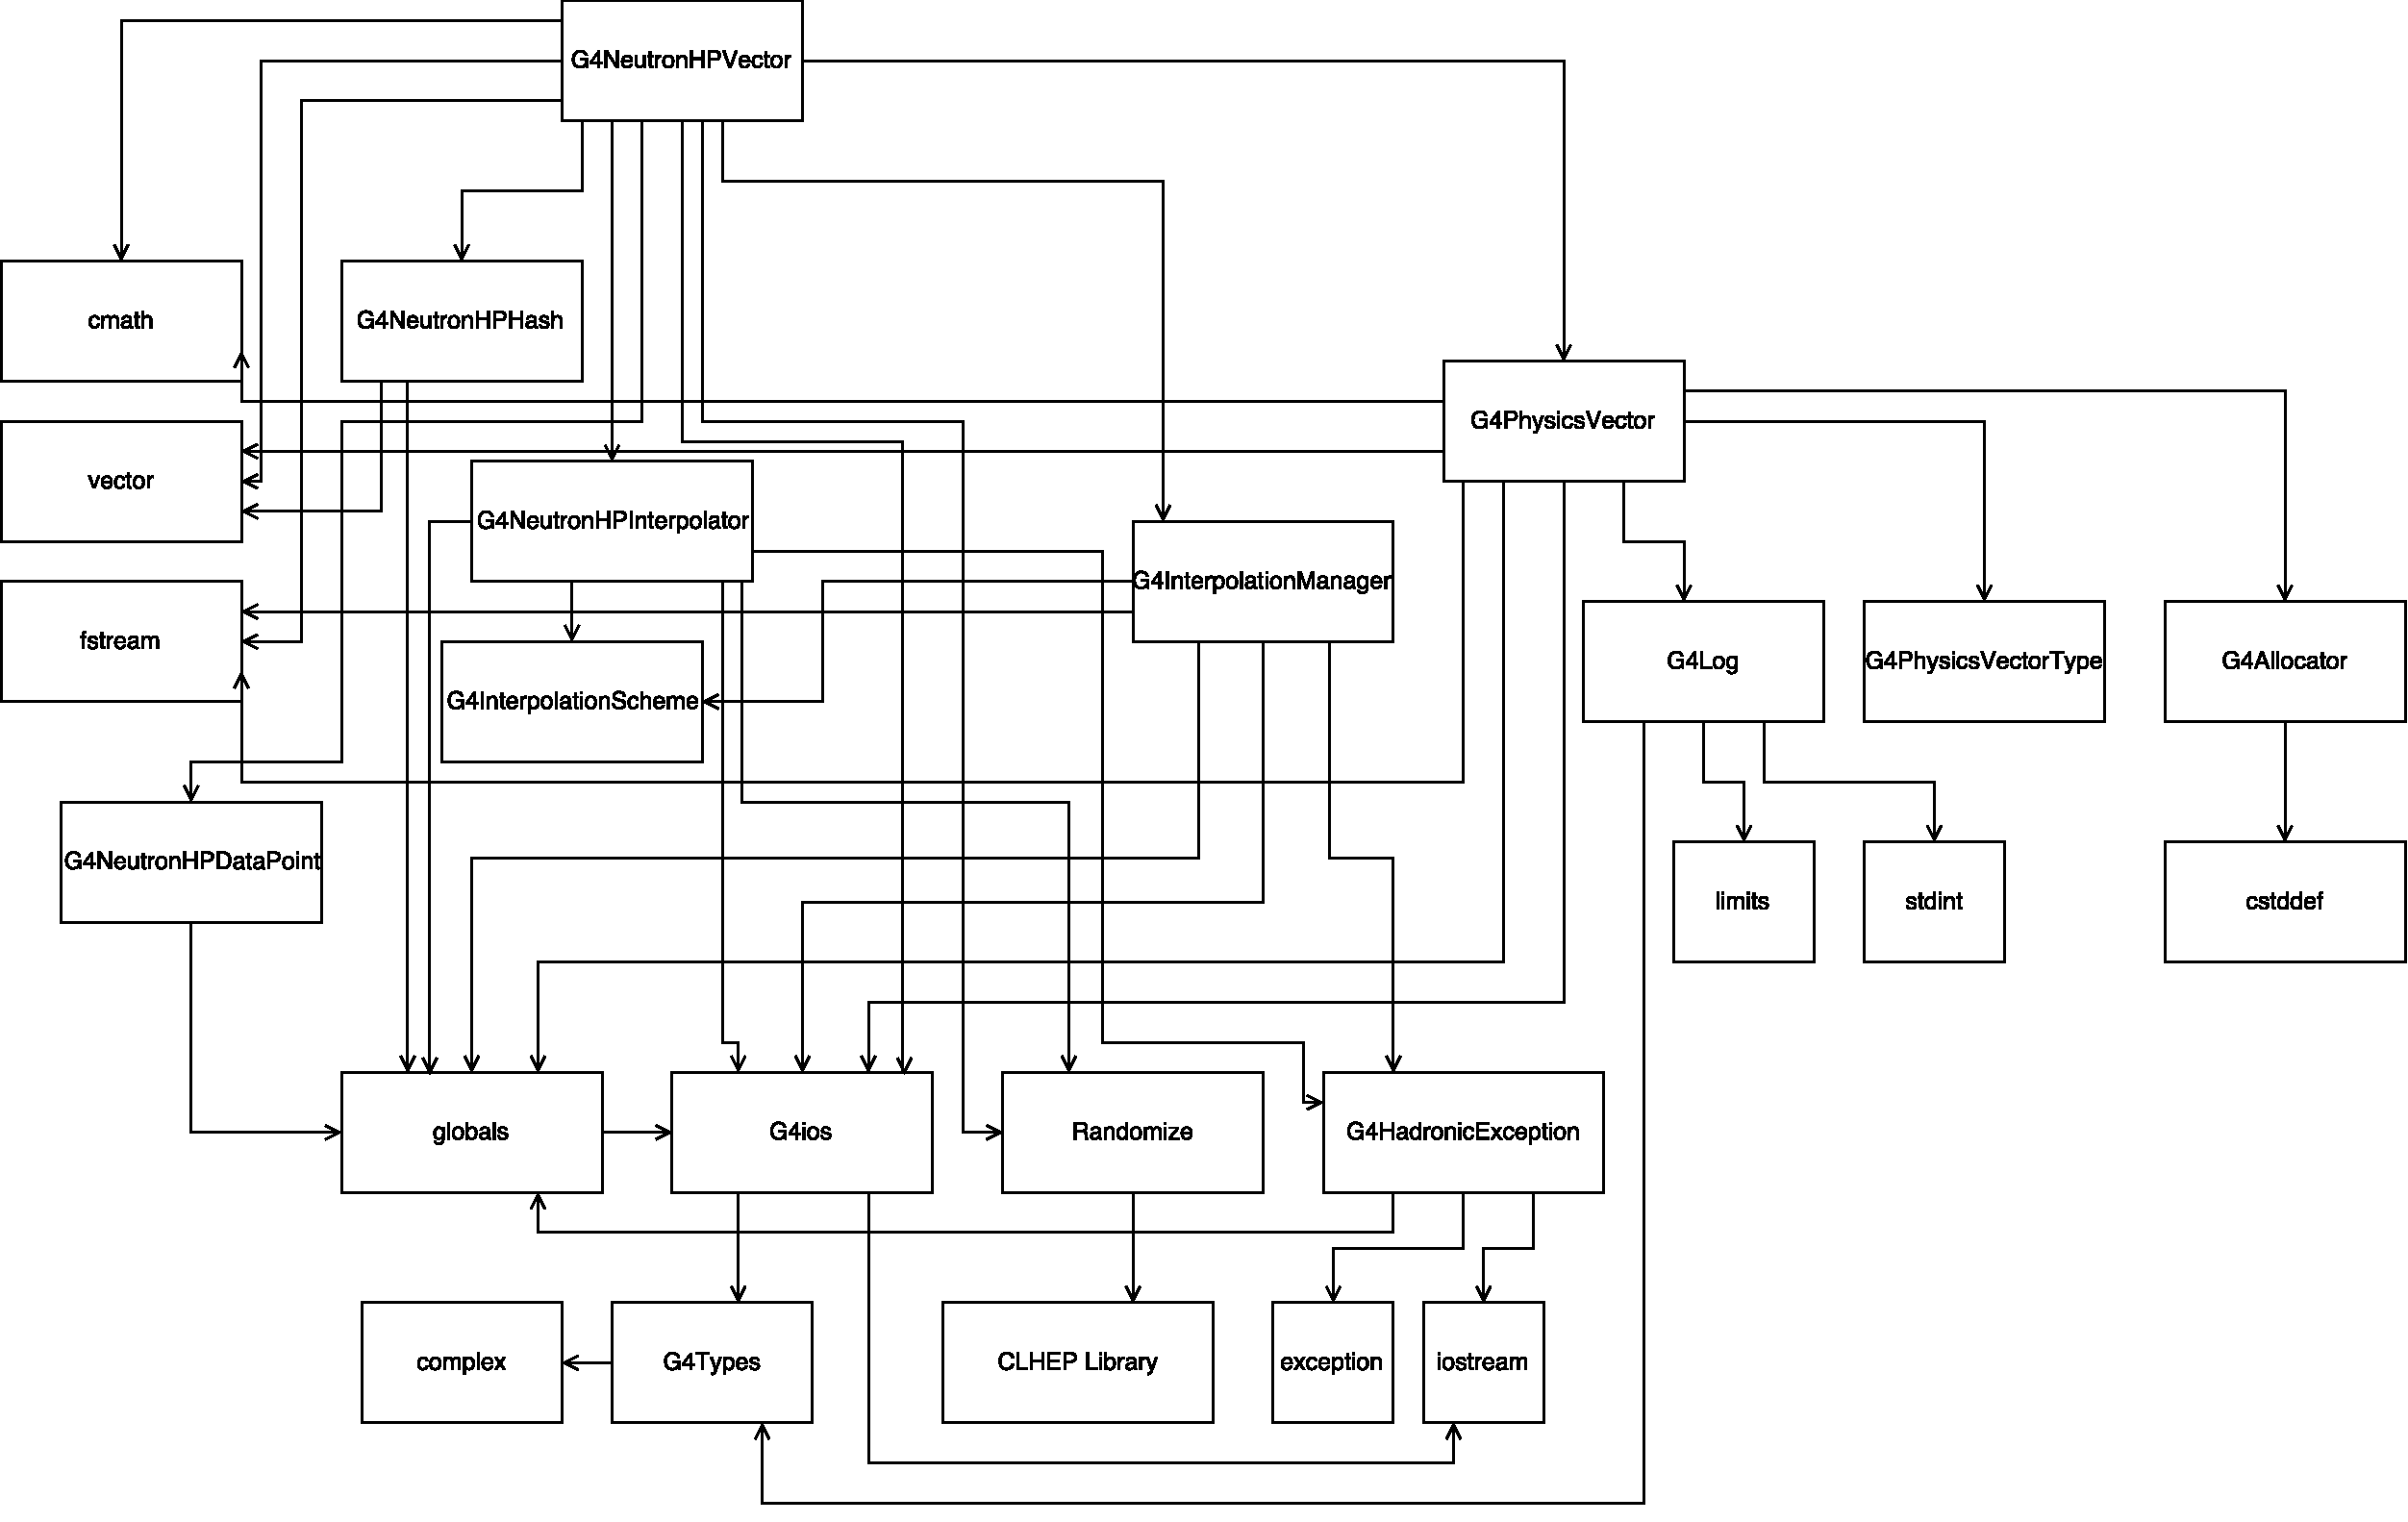
\includegraphics[width=\textwidth]{uses_hierarchy.pdf}
\end{figure}
\FloatBarrier

\section{Traceability of Requirements and Design Components}% ===== Stuart
The following table outlines each requirement and its relationship to the design.

For requirements that do not directly map to sections in the design document (such as providing a repository), the requirement is discussed at a high level in relationship to the design within the context of the entire project.


\begin{center}
\begin{longtable}{>{\raggedright\arraybackslash}p{0.1\textwidth}>{\raggedright\arraybackslash}p{0.3\textwidth}>{\raggedright\arraybackslash}p{0.5\textwidth}}

\caption{Requirements and Design Relationship}\label{Table_RequirementsAndDesign}
\\\toprule
\bf Req. & \bf Description & \bf Design Component\\\toprule
\arrayrulecolor{lightgray}

1  & computations run on GPU & reasoning behind using GPU explained in section \ref{Sec_WhyGPU}. Refer to detailed design document for implementation details.\\\hline

2  & existing projects not affected & by retaining existing code and only calling GPU functions if enabled requirement is met. See section \ref{Sec_IntegrationApproach}.\\\hline

3  & by default simulation will run on CPU & CMake module description in detailed design document explains how this is implemented.\\\hline

4  & should detect if computer has compatible GPU & Detection will be done by CMake, see CMake module in detailed design document.\\\hline

5  & enabling GPU computation on incompatible hardware not allowed & After detection by CMake, an error will be thrown if hardware is incompatible, see CMake module in detailed design document.\\\hline

6  & enabling GPU functionality on existing projects easy & A single boolean flag will be set during CMake phase to enable GPU functionality, see CMake module in detailed design document.\\\hline

7 & runtime of simulation decreased with same output & This is the purpose of the project, and is addressed by porting some computationally-heavy classes to the GPU. Although discussed throughout the design document, particularily relevant sections are sections \ref{Sec_WhyGPU}, \ref{Sec_IntegrationApproach}, and the G4NeutronHPVector module in the detailed design document.\\\hline

8 & accuracy of results same as when run on CPU & Getting the same result whether computation is run on the CPU or GPU is extremely important, and is covered by the internal module design of G4NeutronHPVector in the detailed design document.\\\hline

9 & at least as stable as existing system & Stability again relies on the implementation of the ported modules, specifically the G4NeutronHPVector module from the detailed design document\\\hline

10 & errors will throw exceptions & For each module in the detailed design document a section details how errors will be handled, including the throwing of exceptions\\\hline

11 & will support Geant4 10.00.p02 and later & Currently development is based off of Geant4 10.00.p02. Before the project is made public testing will be done with all major newer versions of the software to ensure compatibility.\\\hline

12 & available on public repo with installation instructions & The project is currently available on a private repo, the installation instructions will be added before the repo is set to public.\\\hline

13 & new versions of product will be available on repo, won't break previous features & All current development is being done with respect to the repository, and changes are all being pushed there. Retaining existing features will be a priority once initial development is complete.\\\hline

14 & all users have access to entire product & This is addressed by the public repository and an upcoming open source license that will be added to the project's documentation.\\

\arrayrulecolor{black}
\bottomrule
\end{longtable}
\end{center}

\end{document}
